\chapter{Выполнение задания}

В этом разделе будут представлены код реализации алгоритма и его графовые представления.


\section{Средства реализации}

В данной работе для реализации был выбран язык программирования \cite{python}.

\section{Программный код}

На листинге \ref{lst:algebr} демонстрируется реализация простого алгоритма DBSCAN. 
\newpage

\captionsetup{singlelinecheck = false, justification=raggedright}
\begin{lstlisting}[label=lst:algebr,caption=Реализация простого алгоритма DBSCAN]
pub fn dbscan(points: &Vec<Vec<bool>>, min_ptx: usize, eps: f64, mut imgbuf: RgbImage) -> u32 {
	
	let mut cluster_count = 0;                         // 1
	let mut current_point = points.clone();           // 2                                            
	for i in 0..points.len() {  						// 3
		for j in 0..points[i].len() {					// 4
			if current_point[i][j] {					// 5
				
				let mut v = Vec::<[usize; 2]>::new();  	// 6
				v.push([i, j]);							// 7
				let mut neighbor_count_check = 0;		// 8
				while !v.is_empty() {					// 9
					let p = v.pop().unwrap();			// 10
					if !current_point[p[0]][p[1]] { 	// 11
						continue;						// 12
					}
					current_point[p[0]][p[1]] = false;	// 13
					
					let mut neighbor_count = 0; 		// 14
					
					regionquery(points, min_ptx, &mut v, &mut neighbor_count, p, eps);		// 15
					
					if neighbor_count >= min_ptx {		// 16
						neighbor_count_check += 1;		// 17
					}
				}
				if neighbor_count_check > 0 { 			// 18
					cluster_count += 1;					// 19
				}
				current_point[i][j] = false;			// 20
			}
		}
	}   
	
	cluster_count
}




\end{lstlisting}


\section{Графовые представления}

На рисунках \ref{oper-1}, \ref{info-1}, \ref{oper-2}, \ref{info-2} представлен операционный граф, информационный граф, граф операционной истории, граф информационной истории.

\begin{figure}[ht!]
	\centering
	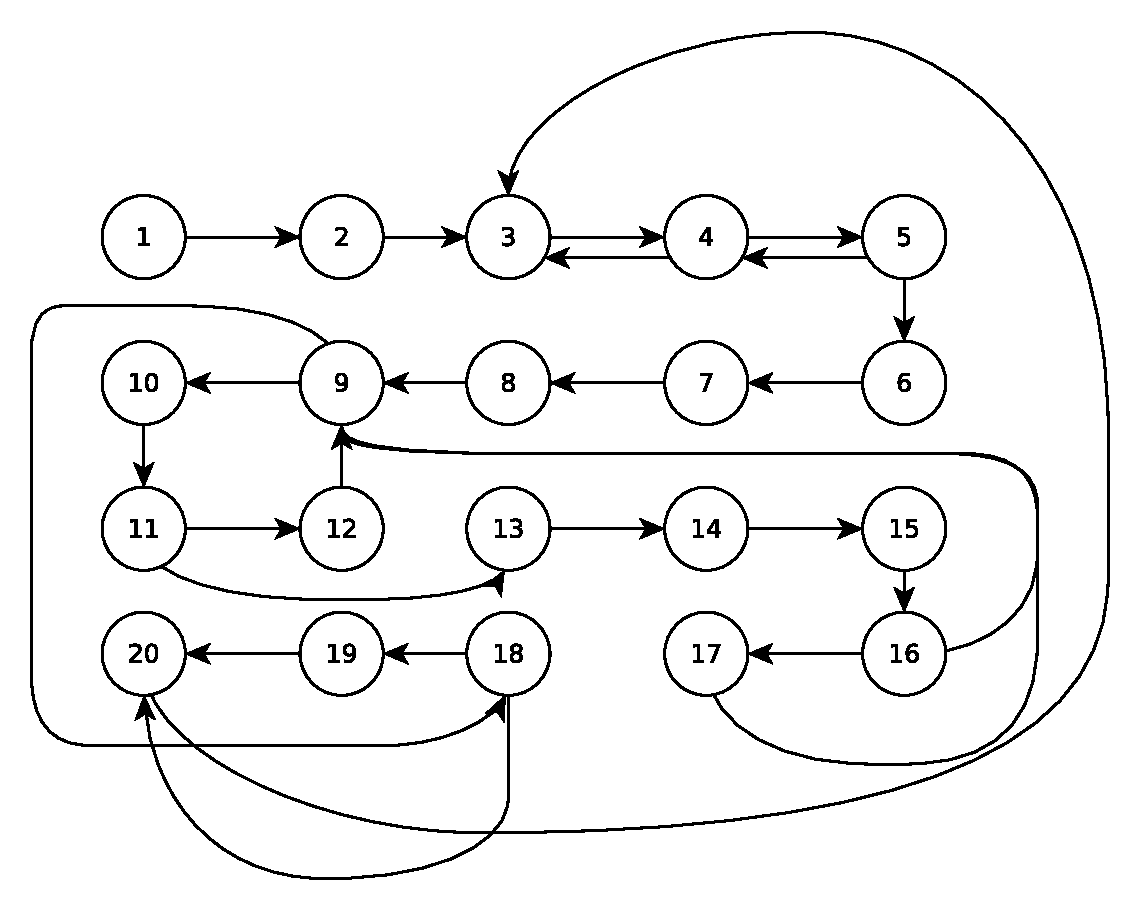
\includegraphics[width=1\linewidth]{assets/graphs/operation.pdf}
	\captionsetup{singlelinecheck = false, justification=centerfirst}
	\caption{Операционный граф}
	\label{oper-1}
\end{figure}
\begin{figure}[ht!]
	\centering
	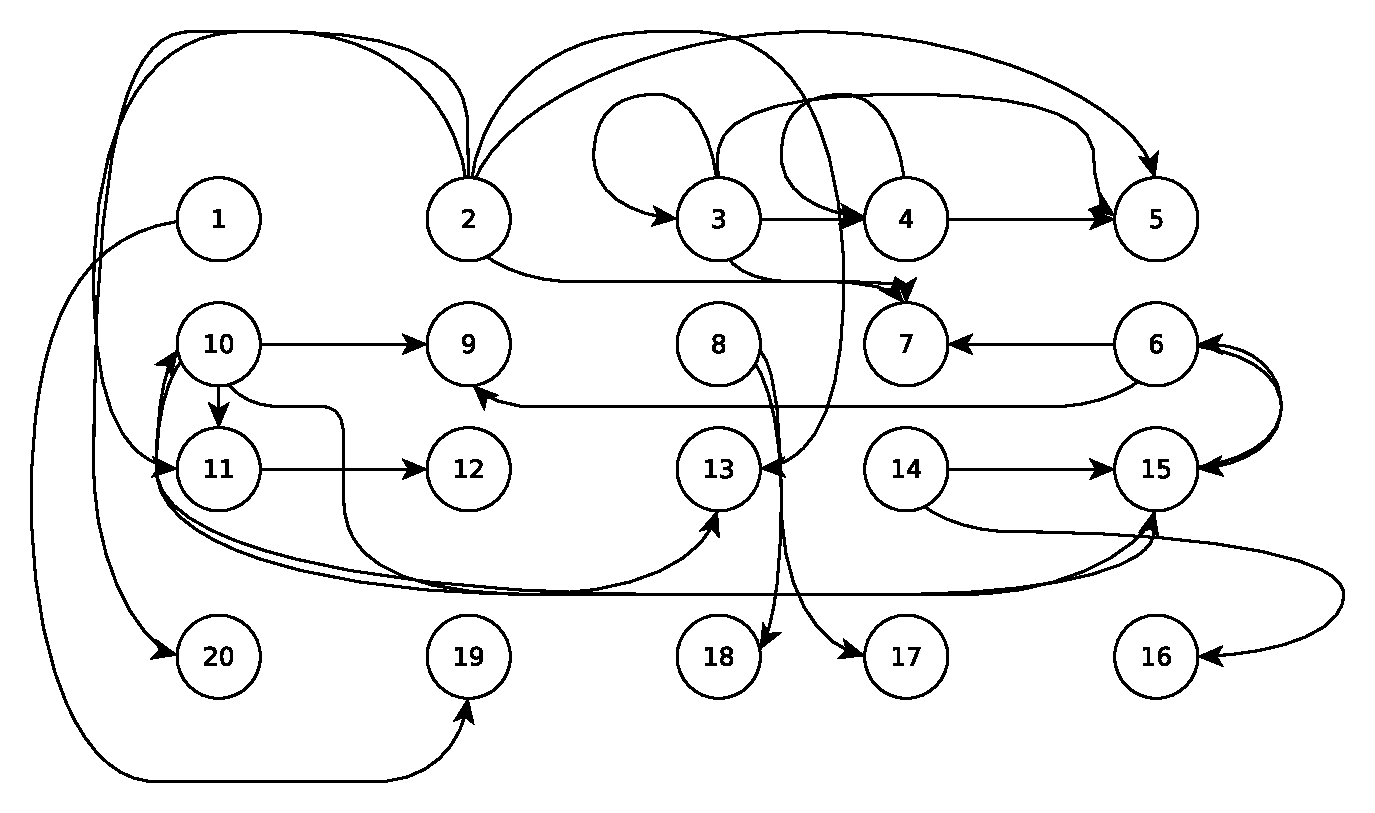
\includegraphics[width=1\linewidth]{assets/graphs/inforamtion.pdf}
	\captionsetup{singlelinecheck = false, justification=centerfirst}
	\caption{Информационный граф}
	\label{info-1}
\end{figure}
\begin{figure}[ht!]
	\centering
	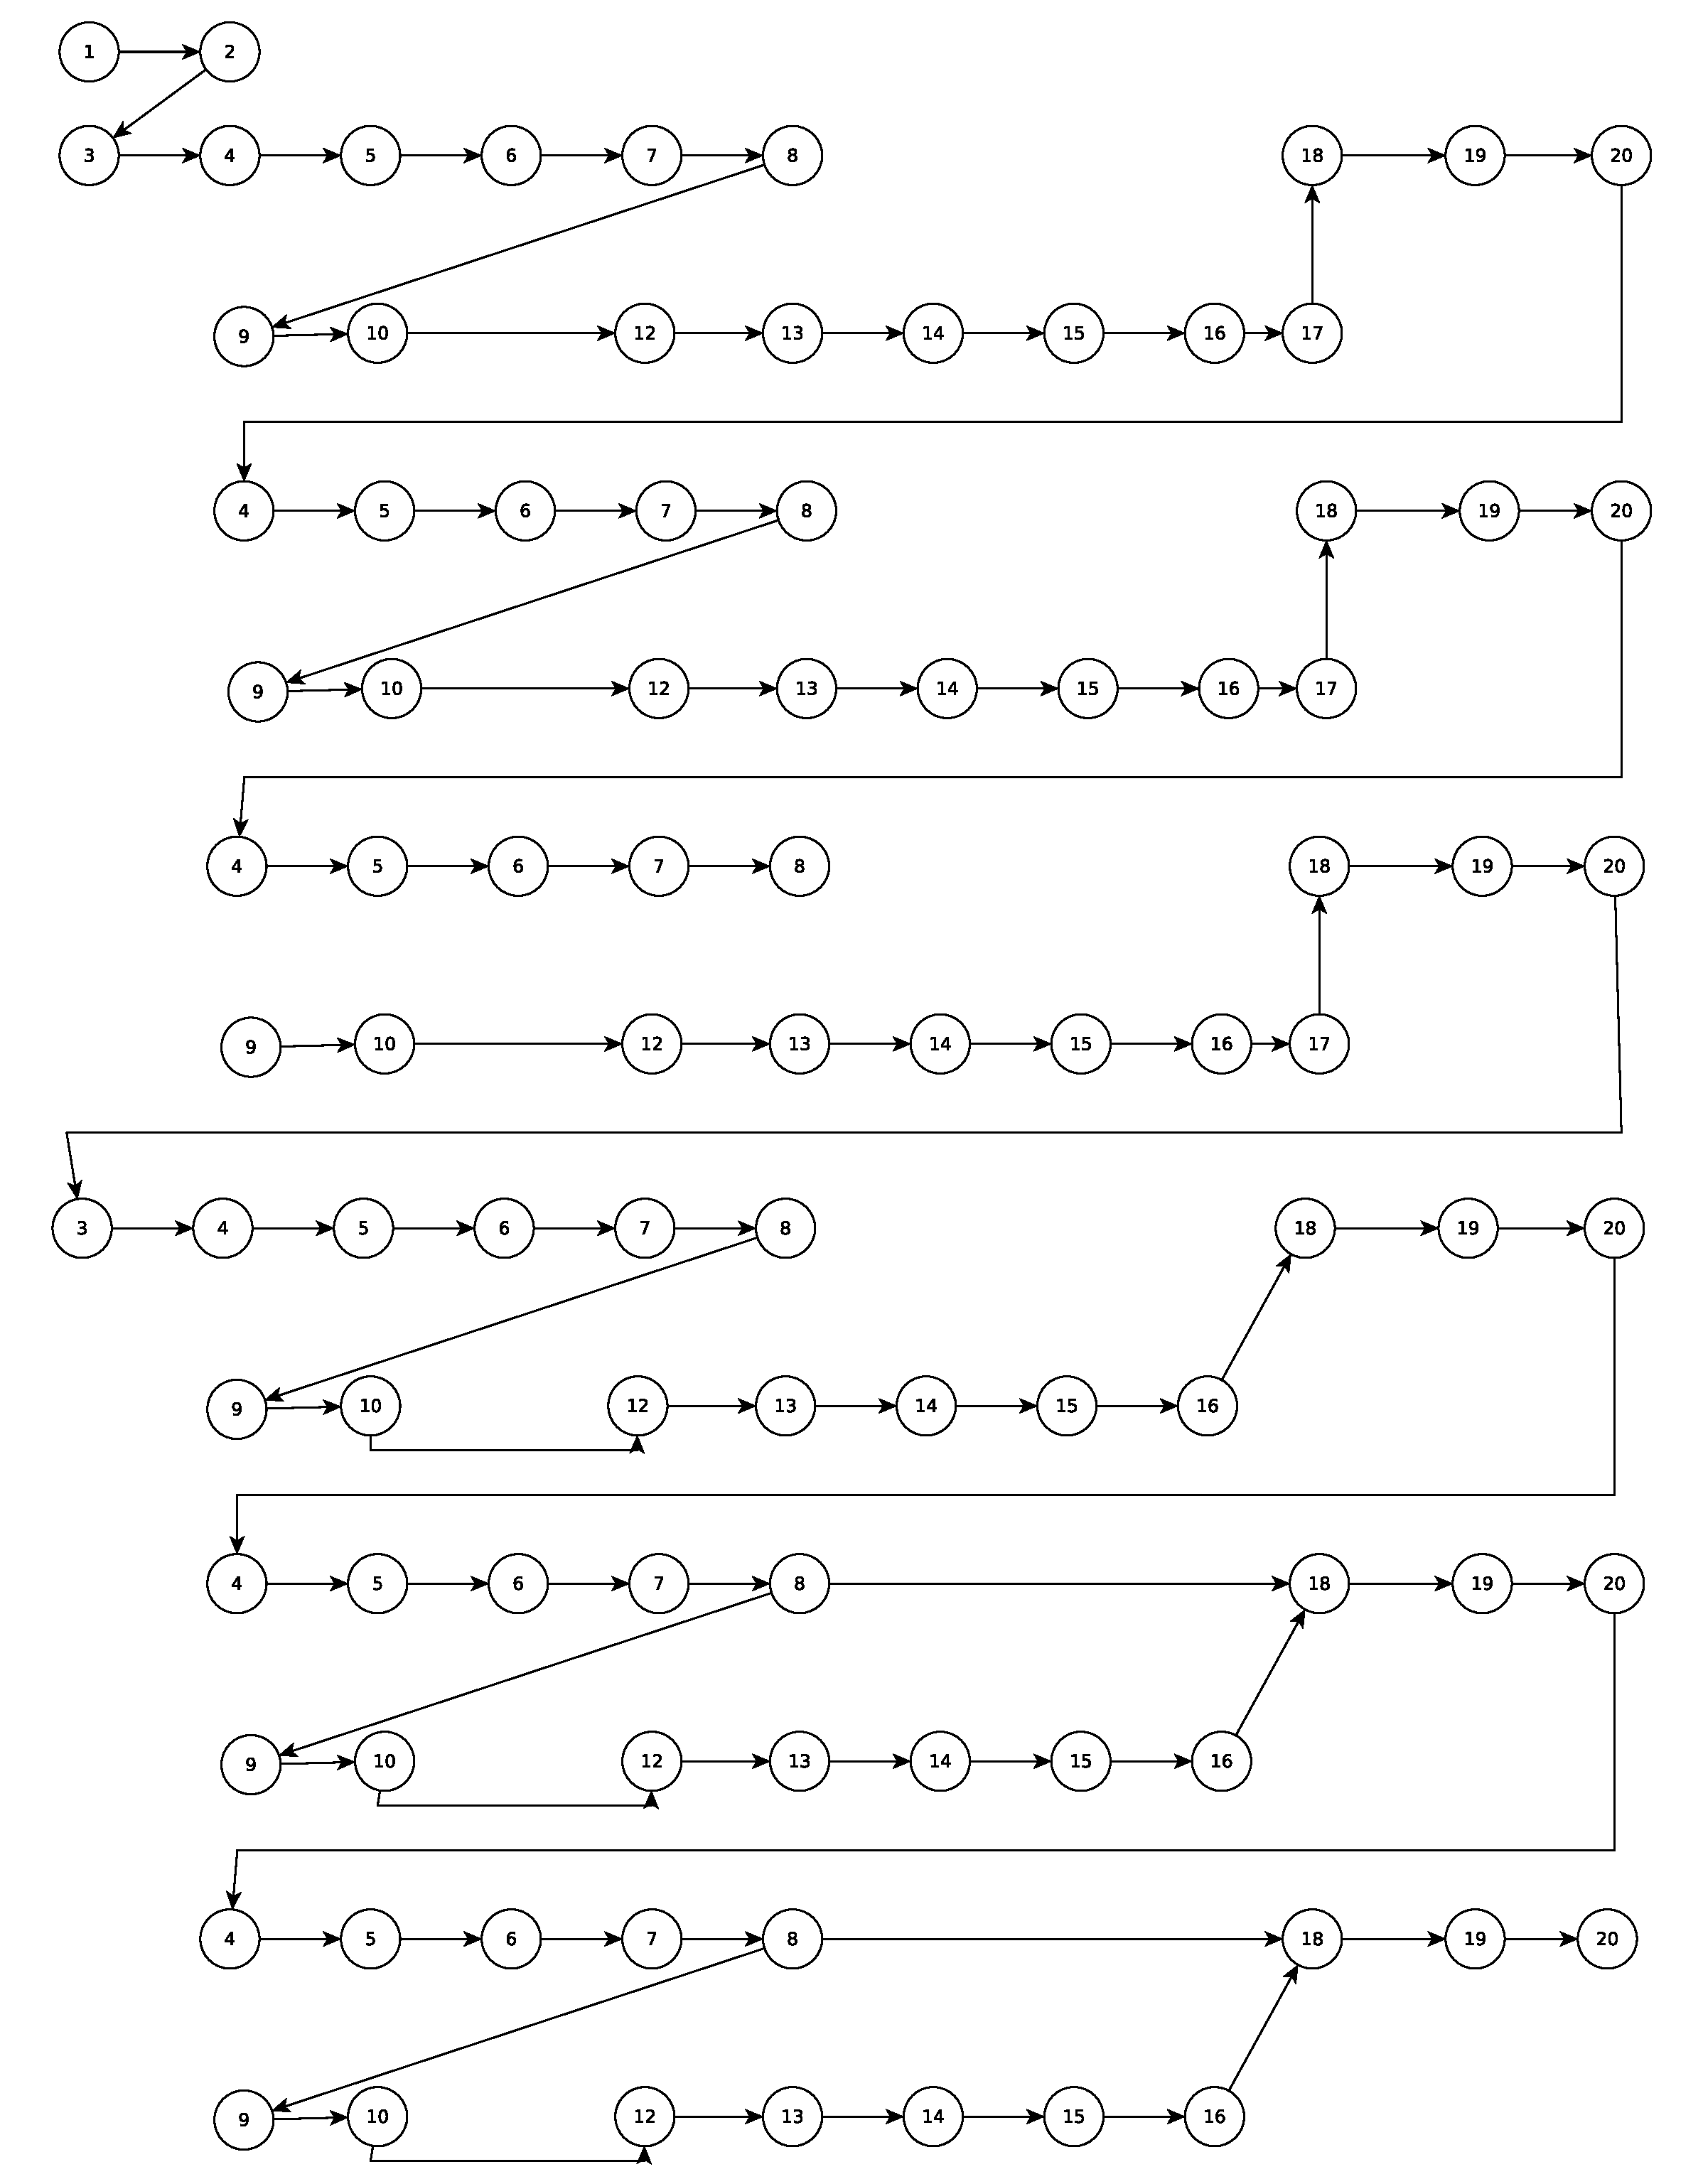
\includegraphics[width=1\linewidth]{assets/graphs/history_operation.pdf}
	\captionsetup{singlelinecheck = false, justification=centerfirst}
	\caption{Граф операционной истории}
	\label{oper-2}
\end{figure}
\begin{figure}[ht!]
	\centering
	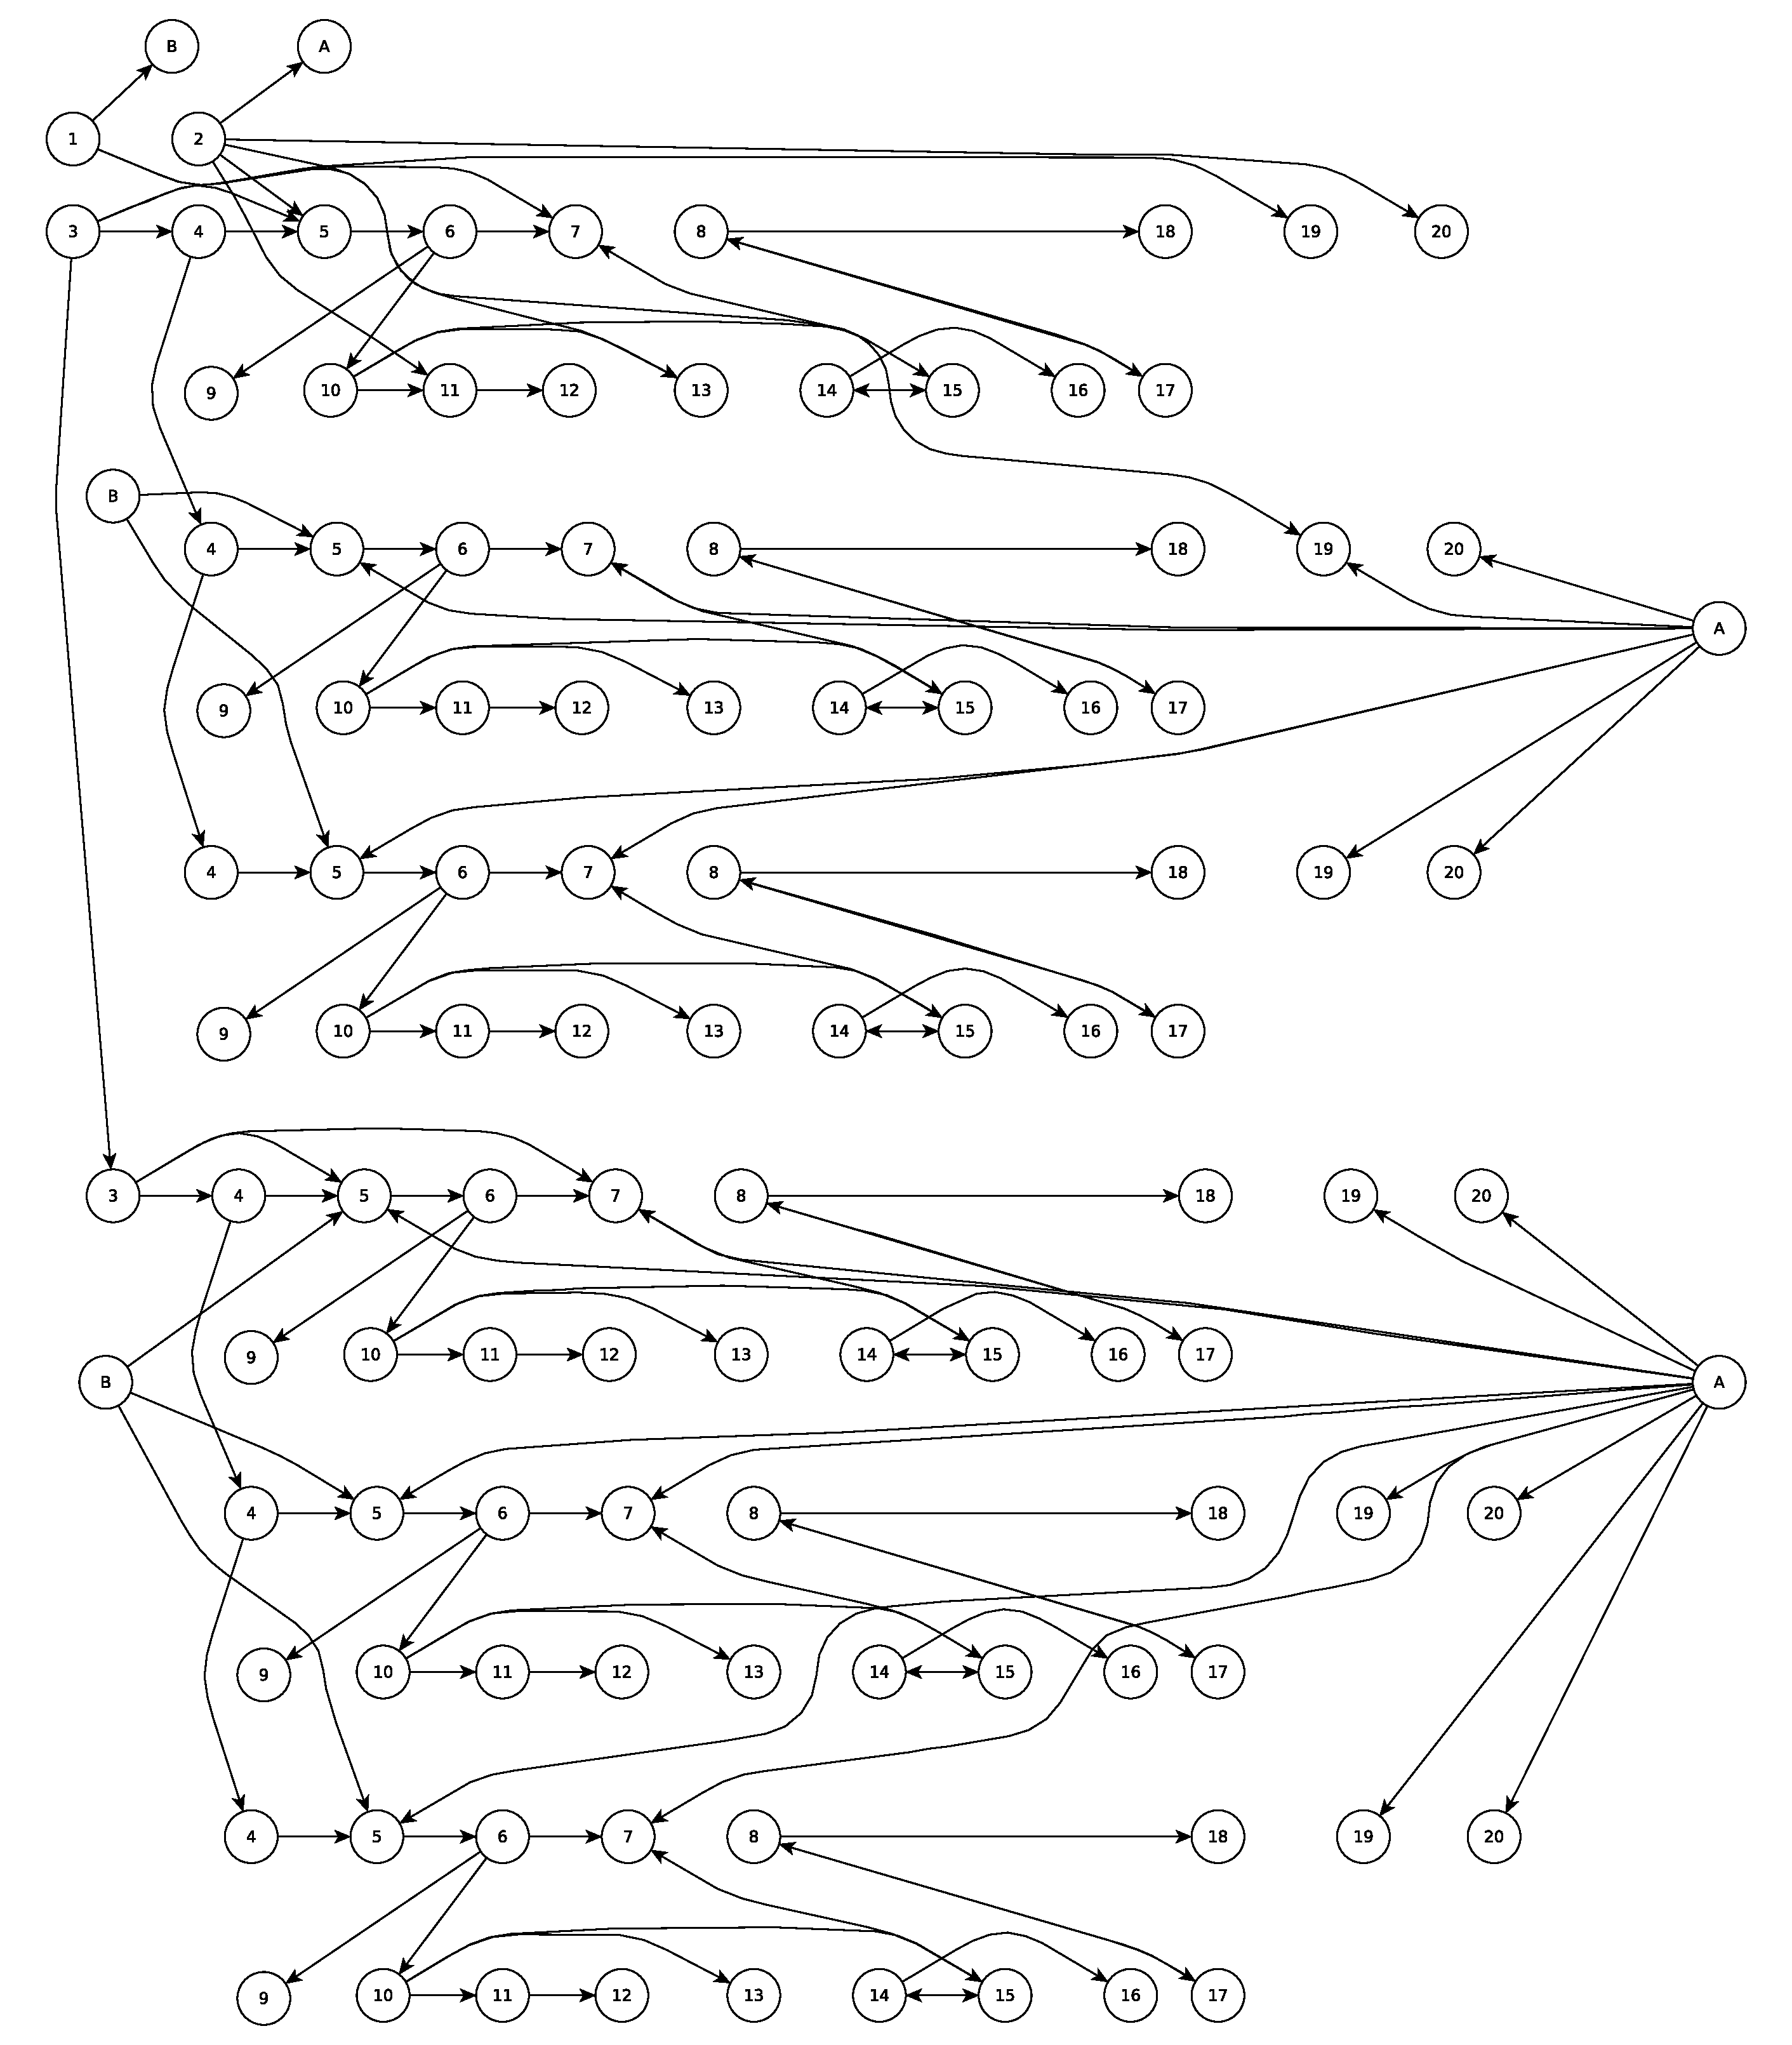
\includegraphics[width=1\linewidth]{assets/graphs/history_information.pdf}
	\captionsetup{singlelinecheck = false, justification=centerfirst}
	\caption{Граф информационной истории}
	\label{info-2}
\end{figure}